\documentclass{article}

\usepackage{amsmath,amssymb}
\usepackage{multicol}
\usepackage{color}
\usepackage[margin=.8in]{geometry}
\usepackage{indentfirst}
\usepackage{hyperref}
\usepackage{framed}
\usepackage{enumerate}

\usepackage{graphicx}
\usepackage{verbatim}


\newcommand{\bigO}{\mathcal{O}}
\newcommand{\CC}{C\nolinebreak\hspace{-.05em}\raisebox{.4ex}{\tiny\bf +}\nolinebreak\hspace{-.10em}\raisebox{.4ex}{\tiny\bf +}}

\definecolor{textcol}{RGB}{0,0,0}

\definecolor{cont}{RGB}{90,20,50}
\definecolor{reach}{RGB}{80,80,80}

\definecolor{abstract}{RGB}{200,100,183}
\definecolor{superclass}{RGB}{210,185,80}
\newcommand{\extends}[1]{ : \textcolor{superclass}{#1}}
\definecolor{filename}{gray}{.25}
\newcommand{\filename}[1]{\texttt{\color{filename}#1}}


\definecolor{macro}{RGB}{98,13,7}
\newcommand{\macro}[1]{\texttt{\color{macro}#1}}

%Itemize

\definecolor{good}{RGB}{20,220,10}
\definecolor{bad}{RGB}{235,10,22}
\definecolor{neutral}{gray}{.75}

\newcommand*\iplus{\item[\textcolor{green}{\textbf{+}}]}
\newcommand*\iminus{\item[\textcolor{bad}{\textbf{--}}]} %TODO \mathlarger ?
\newcommand*\ineutral{\item[\textcolor{neutral}{$\mathbf{\sim}$}]}



\newcommand{\mat}[1]{\mathbf{#1}}



\title {FRaC++ Implementation Design}
\author{Cyrus Cousins}
\date{Fall 2014}

\begin{document}
\maketitle

\begin{multicols}{2}

\tableofcontents
\listoffigures
\par
\bigskip

\begin{framed}
\textbf{Chroma Key:} \\
\color{cont}Controversial Topic \\
\color{reach}Long Term Goal
\color{textcol}
\end{framed}

\end{multicols}

\pagebreak[3]

\section{Introduction}
\label{sec:intro}

\begin{multicols}{2}

\subsection{Motivation}

The current iteration of FRaC \CC{} is poorly organized code of variable quality.  FRaC logic is mixed in with the main program, and the code to deal with SVMs does not have a clear and reusable interface.  Additionally, small amounts of text related code remain in python, and although the performance impact of these is probably negligible, this probably does negatively effects fragility, portability, and maintainability.  Seeing as most of these are design issues, I have decided to create a clear design document for the next iteration of the FRaC \CC{} implementation.

\subsection{Overview}

Section \ref{sec:alg} contains a description of FRaC and all subalgorithms.  Section \ref{sec:obj} contains a description of all the types and interfaces defined in the FRa\CC{} implementation.  Section \ref{sec:arch} contains information on the architecture of the overall algorithm (and possible extensions to it), as well as the architecture of the implementation, including an enumeration of the contents of each source and header file, and also information on external libraries.  Section{sec:scale} describes scalability concerns of this implementation.  Finally, Section \ref{sec:aux} contains design for auxiliary components of the project.

\end{multicols}

\pagebreak[2]

\section{Algorithms}
\label{sec:alg}

\begin{multicols}{2}

FRaC and the algorithms that FRaC uses as subroutines are currently thrown together largely haphazardly.  A modularized design is necessary to create a maintainable and codebase.
 
\subsection{Core Algorithms}
\subsubsection{FRaC}

Currently, FRaC is implemented in \texttt{main.cpp}.  This is in clear violation of separation of concerns and modular software engineering.

\subsection{Feature Reduction Algorithms}

\color{reach}

FRaC thrives on finding patterns of redundancy, and many feature detection techniques eliminate such patterns, and are therefore not useful for FRaC, despite their performance in traditional classification and regression problems\footnote{This is primarily because in FRaC, the training data is not supposed to capture the full variability of the space, but rather only the variability of normative instances.}.  For instance, techniques like eliminating low variance features, removing highly correlated features, and PCA, are all antitechniques in the context of FRaC: the first removes features that are essentially red flags for anomalous instances, the second removes a highly learnable pattern that when violated is an excellent indicator of an anomaly, and the third simplifies the feature space in such a way that a anomalous instances cannot even be expressed.

\subsubsection{Unknown Elimination}

In the most extreme case, if we make the assumption that the existence or nonexistence of a feature is not in and of itself a feature, it can be said that a feature for which no training samples have data provides no information to test samples, so it may be discarded.  On the less extreme end, features for which training data is sparse are more susceptible to noise and overfitting.  The technique of eliminating features for which at least some percentage $p$ of test instances are missing thus reduces the feature space at minimal (tuneable) cost to accuracy.

Many machine learning algorithms are designed to classify very quickly, but often take a long time to train.  Because FRaC and CSAX require the training of a large number of models, feature reduction is especially pertinent.  Feature reduction is not explicitly a part of the FRaC pipeline at this time.

\subsubsection{Low Feature Absolute Value Correlation}

\label{sec:cormat}

The basic algorithm is to generate a correlation matrix between all continuous valued features.  The cost of this operation is $\bigO(n^2)$ time and space, however it is important to note that if training the regressor used requires $\Omega(n)$ time, then FRaC itself requires $\Omega(n^2)$ time, so this will not be the dominant cost.  The storage requirements may however be a concern.  From the correlation matrix, for row (list) \texttt{i}, the value \texttt{sum (map abs i) / (length i)} is taken to be the average absolute value correlation, and the features of all rows with such values under some cutoff $c$ are removed.

Though it is a poor heuristic because the actions of one feature can interact in complex ways with the actions of other features, a feature that does not correlate with any other feature probably is not an effective indicator of any other feature, nor are other features capable of predicting it, therefore the removal of such a feature is an effective optimization at minimal (tuneable) cost to accuracy.  Such removals when done conservatively may even boost accuracy by preventing algorithms from becoming confused by irrelevant features.

\subsubsection{Category Elimination}

Over categorical features, it may be that certain categories are highly similar, or even indistinguishable\footnote{A motivating example: Suppose an SNP has a major allele and 2 minor alleles, but both minor alleles code for redundant codons.  Barring subtle biochemical effects and different binding affinities and/or tRNA densities, \textit{both minor alleles should have identical function}.} by FRaC's trained models.  If a statistically significant difference between categories is not detected, the categories may as well be considered the same.  This has the potential to improve computational performance, convert binary classification problems into unary classification (which of course allows the feature to be eliminated), and multary classification problems to binary classification problems.  In the reduced classification problems, names of categories should clearly and unambiguously represent the original group of categories that were combined.  Furthermore, accuracy may be boosted because rules are more learnable, as essentially the learners have more data for the combined categories.

This technique as written above would require a full cycle of training for each categorical variable to eliminate from, so it may be more effective to use a heuristic, such as average values for other features by class, to determine whether categories differ, or alternatively, training over partial datasets.  Both of these techniques are faster, but introduce the possibility of erroneously eliminating categories that do exhibit meaningful variance.

\color{textcol}

\subsection{Machine Learning Algorithms}

\label{sec:alg:mlalgs}

As a meta algorithm, FRaC uses many component algorithms, which are enumerated below.  Existing implementations are referenced where available.

%\begin{multicols}{2}

\subsubsection{Regression Algorithms}

\begin{enumerate}

\item SVM techniques (libsvm code)
\item Decision tree techniques (Weka code, alternatives when possible)
\item Other techniques...

\end{enumerate}

\subsubsection{Classification Algorithms}

\begin{enumerate}

\item Decision tree techniques
\item Other techniques...

\end{enumerate}

\subsubsection{Binary Classification Algorithms}

\begin{enumerate}

\item SVM techniques
\item Decision tree techniques
\item Other techniques...

\end{enumerate}

\end{multicols}
\pagebreak[2]

\section{Objects and Types}

\label{sec:obj}

\begin{multicols}{2}

As the implementation is in \CC{}, good programming practices for the language are to use objects.  Very little of the framework actually benefits from full polymorphic objects, but even for the sake of data encapsulation and functional abstractions, the use of object oriented technique is, in my opinion, highly valuable.

The convention I am using is to give all primitive types a lower case name succeeded by ``\texttt{\_t}'' (ie \texttt{contvar\_t}), and all classes capitalized names in PascalCasing.

\color{textcol}

\subsection{Sample}

A \texttt{Sample} object represents a single complete data entity, consisting of continuous, discrete, and binary\footnote{One may note that binary values are indeed a form of discrete value.  Many optimizations, both in memory and performance, are possible on binary values, and there exist many binary classification algorithms, so the dual categorization has value.  I believe this value to be enough to complicate the implementation by the introduction of a third value type.}.  In the FRaC literature, conditions for possible datatypes are given, and discrete and continuous values are experimented on.  In the future, more types, such as continuous\footnote{A discrete vector can trivially be represented as a single discrete value in the space of the cross product of the spaces of each dimension, and I do not see motivation to do otherwise.} vector types\footnote{One may wonder as to what the purpose of a continuous vector type is, when we can simply break a vector into multiple continuous values.  Information is lost from continuous vectors when they are normalized separately rather than as a group.  A continuous vector could perhaps be used for a data type representing the differential expression of alternatively spliced transcripts of a single gene.}, may be added should we decide to support such things.

A \texttt{Sample} object has no meaning except in the context of a \texttt{SampleStructure} object, because neither the names of the features nor even their counts are contained in the sample object (this means that a \texttt{Sample} cannot even be \texttt{examined} without the knowledge contained in a \texttt{SampleStructure}).  This design decision was motivated by the need to have numerous \texttt{Sample}s of the same \texttt{SampleStructure}, without sparing the memory to hold this information in each \texttt{Sample}.

Under no circumstance does FRaC mandate that there be more than a single \texttt{SampleStructure}, and it is created when a dataset is loaded.  Because of this, a situation with the potential to be highly confusing should be relatively straightforward.

\subsubsection{Primitive Types}

Here the space of each primitive type in a sample is informally defined, along with the machine types that will be used to represent or approximate them.

\begin{itemize}

\item \texttt{contvar\_t} = $\mathbb{R} | \textsc{Unknown}$

Represented as a floating point type, with \texttt{NaN} filling in as \textsc{UNKNOWN}.  A \texttt{contvar\_t} represents a continuous feature variable.

\item \texttt{catvar\_t} = $z \in \mathbb{Z}_{2^n-2} | \textsc{Unknown}$

For some $n$ being the number of bits, the categorical type is represented as an unsigned integer of $n$ bits such that the max value ($2^{n}-1$) represents an unknown type.  A \texttt{catvar\_t} represents a categorical feature variable.

\item \texttt{binvar\_t} = $0 | 1$

Wherever possible, these variables will be represented as single bits\footnote{In the petabyte world of today, such representations of bits are often considered \textit{hacks} when seen outside of, say, kernel code.  To offer a motivating example, in the proposed work on allele variations, many alleles are represented as major or minor.  With 1000 samples of a SampleStructure of 10,000 genes, 7,000,000, or 70mb, are saved with this representation.  The implications for locality sensitive regions of code are potentially enormous.} in a bitvector.  This leaves no representation for \textsc{Unknown}, mandating\footnote{Alternatively, we could sacrifice a second bit per value to the ``knownity'' of each value, or, say, store 5 ternary values in 8 bits ($3^5 = 243 < 256 = 2^8$) or similar.  However, this implementation has the advantage of a fast enumeration of all unknown indices \textit{without mandating iteration} of all values.}  the addition of an array of integers, representing unknown indices, to be packed along \texttt{binvar\_t}s.  A \texttt{binvar\_t} represents a binary feature variable.

\end{itemize}

\par\bigskip

Data Representation:

\texttt{type Sample = Sample contvar\_t* catvar\_t* binvar\_t* Array<int>}

\par
\bigskip

\color{cont}
Alternatively, it is less memory efficient but does not require a traversal of the entire sample at unknown value inference time if a list of unknown values is maintained for each feature type.  This also has the advantage that it can track values that had been unknown but were later filled.  This list can be converted to a hash lookup, or, since the logical manner of constructing a list already produces a sorted list of indices, it can be used for binary searches to determine if a value was or was not originally known.

\color{textcol}


\subsection{SampleStructure}

A \texttt{SampleStructure} object represents the number of each primitive \texttt{Sample}s of the \texttt{SampleStructure} have, as well as their names.  A \texttt{SampleStructure} provides the context under which a \texttt{Sample} or a \texttt{Predictor} can be examined.

\par\bigskip
Data Representation:

\texttt{type SampleStructure = SampleStructure String* int int int}

\par
\bigskip

\subsection{StructuredSampleCollection}

A \texttt{StructuredSampleCollection} is basically a convenient wrapper for a \texttt{SampleStructure} and a sized array of \texttt{Sample}s.  This encapsulates all the data necessary to operate on a dataset in a highly concise manner\footnote{Note that no information is repeated in a \texttt{StructuredSampleCollection}: the schema of the \texttt{Sample}'s are represented once in the \texttt{SampleStructure} object, and the \texttt{Sample}'s themselves are packed in an unboxed sized array (of type \texttt{Array<Sample>}).}.  This object provides functionality over datasets, such as validation functions, normalization, and unknown value inference.

\subsection{Predictor}

The predictor type holds classifiers and regressors for all the \texttt{Sample}s of a certain \texttt{SampleStructure}.  For different definitions of ``normal'', the same \texttt{SampleStructure} could theoretically have multiple corresponding \texttt{Predictor}s, but such does not occur at this time in the FRaC framework.  The structure of a \texttt{Predictor} is like that of a \texttt{Sample}, where a value of type \texttt{v} is replaced by a learner with a function of type \texttt{(SampleStructure, Predictor) -> v}.

\par\bigskip

The predictor supports the following operation for a \texttt{Sample} of the same \texttt{SampleStructure}:

\texttt{predict = (Regressor, Sample) -> Sample}

Here the output \texttt{Sample} is the prediction.  Finally, the most straightforward predictor constructor is simply:

\texttt{construct = (SampleStructure, Sample[], (SampleStructure, Sample[], int) -> Regressor, (SampleStructure, Sample[], int) -> Classifier, (SampleStructure, Sample[], int) -> BinaryClassifier) -> Predictor}

Wherein the three arrow typed arguments are simply constructors for a regressor, a classifier, and a binary classifier, respectively.  This technique alleviates the need for a common constructor for each machine learning type (discussed in the subsequent section), and in \CC{} can be implemented using function pointers and/or lambda syntax.  Alternatively, they could also be implemented using generic typing.

The constructor simply uses the provided lambdas to train their corresponding learner objects, and do so for each feature in the \texttt{SampleStructure}, using the \texttt{Sample}s provided as ``normal'' instances.

\par\bigskip
Data Representation:

\texttt{type Predictor = Predictor Regressor* Classifier* BinaryClassifier*}

\subsection{Machine Learning Types}

The machine learning types are the domain under which the polymorphism of \CC{} becomes a great asset.  Here only the interfaces for these types are described.

\textbf{Informal type descriptions}
\begin{enumerate}

\item Regressor

Construct: \texttt{SampleStructure Sample[] int -> Regressor}

Regress: \texttt{Regressor SampleStructure Sample -> contvar\_t}

\item Classifier

Construct: \texttt{SampleStructure Sample[] int -> Classifier}

Classify: \texttt{Classifier SampleStructure Sample -> catvar\_t}

\item BinaryClassifier

Construct: \texttt{SampleStructure Sample[] int -> BinaryClassifier}

Classify: \texttt{BinaryClassifier SampleStructure Sample -> bool}

\end{enumerate}

In these interfaces, the integer in the constructor represents the index of the feature to regress on or classify.  Also note that \texttt{SampleStructure} is needed for the learner being constructed to identify the width of each feature type's array in the \texttt{Sample}s.  

Finally, note that these constructors are only approximate: for good reasons, constructor interfaces do not exist in \CC{}, and different machine learning types will require different information (generally parameteterizations) to construct.  To circumvent this limitation, a \texttt{Predictor} may be passed function pointer to create and train a learners of the above three types.


\subsection{Error distribution types}

\label{sec:edisttypes}

The purpose of an error distribution type is to provide a probability distribution to answer queries of the form $P($obs $A|$ true $B)$.

Error distribution types are important in FRaC, and models for each of continuous, categorical, and binary feature types need be implemented.

\textcolor{cont}{For some of these types it is just as natural to store normalized surprisal scores as it is to store probabilities from which to calculate normalized surprisal; this is potentially a powerful optimization.}  The types of a lambda function taking observed $a$ and actual value $b$ of the probability and the normalized surprisal are as follows: 

\begin{verbatim}
probabilityObsAExpB :: a -> b -> real
normalizedSurprisalObsAExpB :: a -> b -> real
\end{verbatim}

Note that these functions are identically typed, the normalized surprisal simply has more information in it.  By creating error models that directly model normalized surprisal, we cut out an extra layer of potentially confusing architecture.

\subsubsection{Gaussian}

Implemented as a struct in the original \CC{} implementation, the Gaussian is a simple but fast error distribution.  It is incapable of representing many complex but realistic situations.
%\subsection{Other FRaC types}

\color{reach}
\subsubsection{Bucketized error distribution}

Implemented in the python version of FRaC, bucketized error representations require more data to create and can overfit relative to gaussians, but are capable of modeling more complex spaces.
%\textcolor{red}{Value distribution types have yet to be defined.} 

\color{textcol}

\subsubsection{Confusion Matrix}

The confusion matrix is the natural representation of an error model for categorical data.  The cells of the matrix may be replaced with normalized surprisal values, and this normalized surprisal matrix can more efficiently serve normalized surprisal queries.  

\color{cont}

In addition to the confusion matrix, it may be worth implementing a half confusion matrix, which for some confusion matrix $\mat{C}$ is given by $\frac{\mat{C} + \mat{C}^T}{2}$.  Half confusion matrices can be easily represented in half the memory of full matrices, and are also less prone to sampling error.

\color{textcol}

\subsubsection{Binary Confusion Matrix}

Over binary data, a simple $2 \times 2$ confusion matrix effectively models the data.  There is great value in having this as a separate type, as it is both more efficient (as with any statically sized matrix) and requires a lower memory footprint\footnote{Many applications, such as major/minor allele based data, deal primarily in binary confusion matrices.  A large number of these represents a significant reduction in memory cost.}.  Furthermore, it is far simpler to implement a binary confusion matrix without indirection, which is again a large performance and memory gain.  Additionally, from a types perspective, as \texttt{BinaryClassifier} and \texttt{Classifier} are separate types, despite the fact that many \texttt{BinaryClassifier}s are really \texttt{Classifier}s in disguise.

\subsection{Error Model Collection}

The \texttt{ErrorModelCollection} type is to the machine types discussed in section \ref{sec:edisttypes} as the \texttt{Predictor} type is analogous to the \texttt{Regressor}, \texttt{Classifier}, and \texttt{BinaryClassifier} types: an \texttt{ErrorModelCollection} is simply a collection of error models of these three types, and is used in calculations of normalized surprisal.  Like the predictor type, it must be interpreted in the context of a \texttt{SampleStructure} object.

\par\bigskip
Data Representation:

\texttt{type ErrorModelCollection = ErrorModelCollection Gaussian** ConfusionMatrix** BinaryConfusionMatrix**} %TODO replace these with cross product type notations.

\end{multicols}
\pagebreak[2]

\section{Architecture}

\label{sec:arch}

\begin{multicols}{2}

\subsection{Graphical Overview of Modular Object Creation and Processing}

\begin{figure*}

%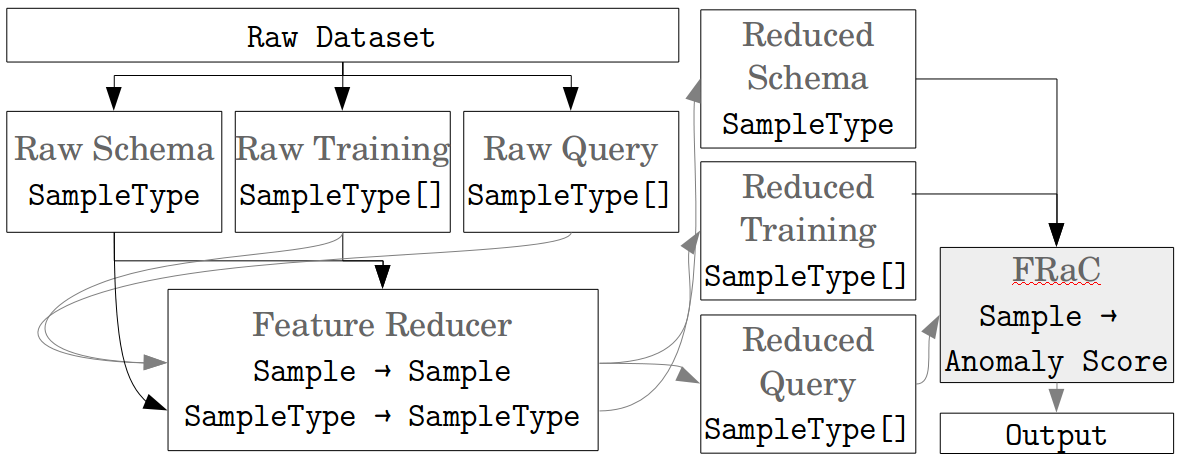
\includegraphics[width=6.7in]{fracpipeline}
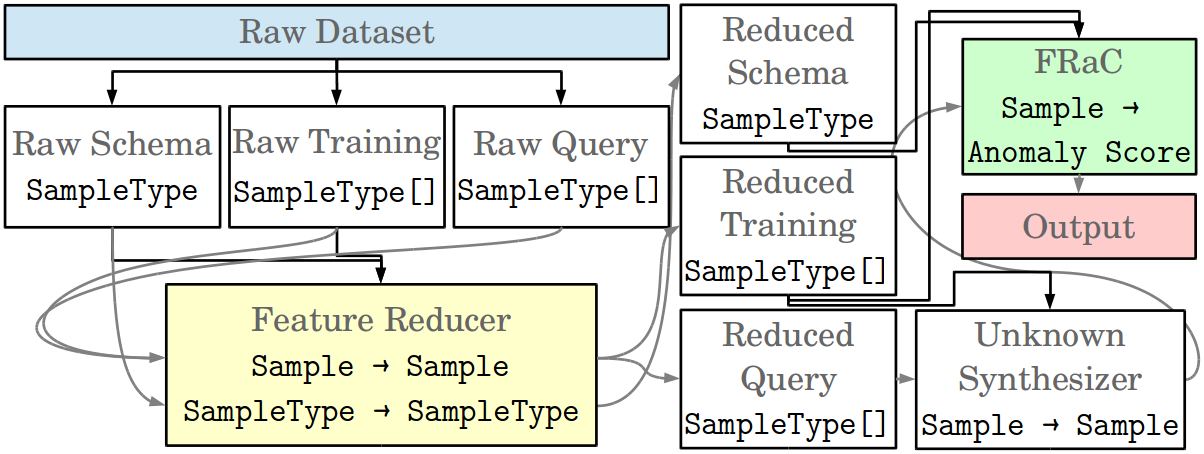
\includegraphics[width=6.9in]{objects3}

\textit{In this diagram, black angular arrows represent creation of an object, and smooth gray arrows denote processing of an object.}

\caption{FRaC extended pipeline.}

\label{fig:pipeline}

\end{figure*}

The FRAC pipeline extended with feature selection is presented in Figure \ref{fig:pipeline}.  

\subsection{Implementation Specific Architecture}

This subsection details the implementation details of the \CC{} implementation itself, including the contents and organization of source and header files.

%TODO: Dependency graph?

\subsubsection{Generic Interfaces and Headers}

\begin{itemize}

\item \texttt{array.hpp} This header contains a very simple generic array type designed to mimic the sized arrays of languages like Java or C\#.  It can largely be considered syntactic sugar to prevent passing array pointers with size integers, though several higher order array operators are provided as well.  A bit array implementation is also provided.

\item \texttt{vectormath.hpp} This is a generically typed header providing basic mathematical functionality over vectors.  Vector here refers to vector in the mathematical sense, not in the perverse sense that the creators of the \CC{} STL intended it.  As a result, most functions in this class are of the form \texttt{(T*, uint) -> T} (or similar).

\item \texttt{types.h} This C header contains definitions that specify the actual machine types used by the FRa\CC{} implementation.  Here the width of the categorical variables and floating point numbers are defined.  This header is fully C99 compatible.

\end{itemize}

\subsubsection{Classes and Modules}

\label{sec:arch:code}


\begin{figure*}

\begin{multicols}{3}
\begin{enumerate}
\item \textcolor{superclass}{Inherits from} (parent class).
\item \textcolor{abstract}{Abstract class} (contains virtual function(s)).
\item \textcolor{filename}{File name}.
\end{enumerate}
\end{multicols}

\caption{Source file chroma key}
\label{fig:sfck}
\end{figure*}

Here the contents of the various FRaC specific source files is presented.  When both a source file and a header file exist, \filename{module.*pp} is written.  See Section \ref{sec:obj} for a description of all objects referenced, and see Figure \ref{fig:sfck} for an explanation of the color scheme used below.

%\begin{multicols}{2}
\begin{itemize}
\item \texttt{main.cpp}
\begin{itemize}
\item Main program logic and overall architecture.
\item Command Line Interface.
\begin{itemize}
\item Help
\item Set learner options
\item View compiled options
\end{itemize}
\end{itemize}
\item \filename{ errormodel.*pp} Error model types.
\begin{itemize}
\item \texttt{\color{abstract}ContinuousErrorModel}
\item \texttt{\color{abstract}CategoricalErrorModel}
\item \texttt{\color{abstract}BinaryErrorModel}
\item \texttt{Gaussian\extends{ContinuousErrorModel}}
\item \texttt{Error\_Bucketized\extends{ContinuousErrorModel}}
\item \texttt{Confusion\_Matrix\extends{CategoricalErrorModel}}
\item \texttt{Normalized\_Surprisal\_Matrix\footnote{Some of the variants of FRaC (such as AP FRaC mentioned in \cite{frac11}) require explicitly intermediate calculation values, which the raw confusion matrix cannot provide.}\extends{CategoricalErrorModel}} %TODO this citation stuff.
\item \texttt{Confusion\_Matrix\_Half\extends{CategoricalErrorModel}}
\item \texttt{Normalized\_Surprisal\_Matrix\_Half\extends{CategoricalErrorModel}}
\end{itemize}
\item \filename{errormodelcollection.*pp}
\begin{itemize}
\item \texttt{ErrorModelCollection} %TODO write about this type...
\end{itemize}
\item \filename{frac.*pp}
\begin{itemize}
\item \texttt{\color{abstract}FRaC}
\item \texttt{TraditionalFRaC}
\item \texttt{APFRaC}
\item \texttt{DiscreteFRaC}
\item \texttt{ProbabilisticFRaC}
\end{itemize}
\item \filename{sample.*pp}
\begin{itemize}
\item \texttt{Sample}
\item \texttt{SampleStructure}
\item \texttt{StructuredSampleCollection}
\end{itemize}
\item \filename{predictor.*pp}
\begin{itemize}
\item \texttt{Predictor}
\end{itemize}
\item \filename{mltypes.*pp}
\begin{itemize}
%\begin{multicols}{2}
\item \texttt{\color{abstract}Regressor}
\item \texttt{\color{abstract}Classifier}
\item \texttt{\color{abstract}BinaryClassifier}

\item \texttt{RegressorConstant\extends{Regressor}}
\item \texttt{ClassifierConstant\extends{Classifier}}
\item \texttt{BinaryClassifierConstant\extends{BinaryClassifier}}

\item \texttt{RegressorEnsemble\extends{Regressor}}
\item \texttt{ClassifierEnsemble\extends{Classifier}}
\item \texttt{BinaryClassifierEnsemble\extends{BinaryClassifier}}
%\end{multicols}
\end{itemize}
\item \filename{waffles.*pp}
\begin{itemize}
\item \texttt{WafflesDecisionTreeClassifier\extends{Classifier}}
\item \texttt{WafflesDecisionTreeRegressor\extends{Regressor}}
\item \texttt{WafflesNeuralNetworkClassifier\extends{Classifier}}
\end{itemize}
\item \filename{svm.cpp svm.h svm-predict.c}
\begin{itemize}
\item Code interfacing with libsvm.
\item Wrapper types for libsvm objects.
\end{itemize}
\item \filename{test.*pp}
\begin{itemize}
\item Basic test functions for various classifiers, \texttt{Sample} functions, \texttt{Predictor}s, error models and \texttt{ErrorModelCollection}s, and the FRaC algorithm itself.
\end{itemize}
\item \filename{io.*pp}
\begin{itemize}
\item Bidirectional conversion between ARFF files and \texttt{StructuredSampleCollection}s.
\end{itemize}
\item \filename{svmlearner.*pp}
\begin{itemize}
\item \texttt{SvmRegressor\extends{Regressor}}
\end{itemize}

\begin{comment}
\begin{itemize}
\item YaDT.h
\begin{itemize}
\item Yet another Decision Tree builder header file.
\end{itemize}
\end{itemize}
\begin{itemize}
\item dTcmd.cpp
\begin{itemize}
\item Yet another Decision Tree builder implementation.
\end{itemize}
\end{itemize}
\end{comment}

%\item \texttt{types.h}
\end{itemize}
%\end{multicols}

\subsubsection{Libraries}

\begin{figure*}

\begin{itemize}
 
\item \textbf{LibSVM}: Support Vector Machine implementations.

\end{itemize}

Candidate Libraries: The following competing libraries are popular \CC{} libraries for general purpose machine learning.  I could not find a good comparison of these libraries, so the data presented here are solely from my own early impressions.  The pros and cons of each are discussed here.

\begin{itemize}

\item \href{http://ai.stanford.edu/~ronnyk/mlcHB.pdf}{ML\CC{}} (4140 hits)

\begin{itemize}

\iplus Free for research use.

\iplus Extremely mature (documentation is from 1996).

\iplus C4.5 decision trees.

\iminus Popularity seems to be low today.  Perhaps the software is past its peak.

\iminus Does not seem to want to be consumed as a library.  ML\CC{} seems to want to be an independent program, it may have a very difficult API.

\end{itemize}

\item \href{http://dlib.net/}{Dlib} (7000 hits)

\begin{itemize}

\iplus Mature.

\iplus Well documented: ``I consider the documentation to be the most important part of the library.''

\iplus High portability: no dependencies, and OS abstraction wherever necessary.

\iplus Multithreading

\iplus SVM, RVM, multiclass SVM with linear kernel, binary classifiers.

\iminus \textbf{No decision trees.}

\end{itemize}

\item \href{http://image.diku.dk/shark/sphinx_pages/build/html/index.html}{Shark} (63900 hits)

\begin{itemize}

\iplus Popular (though this could be inflated due to the popularity of the word ``Shark''.

\iplus SVM, neural network, radial basis function networks, decision trees w/ random forests.

\iplus Shark is intended to be statically linked.

\iplus Mature (~10 years)

\ineutral Obscure algorithms are implemented in Shark.  Many interesting algorithms are there, but perhaps more mainstream algorithms would be useful for FRaC.

\iminus Requires Boost.

\iminus Build is a pain, requires CMake, and has a bizarre multi tier build complete with an ``installation''.  Having to build Shark will massively complicate builds (install Boost headers, install CMake, build several things...), which may reduce cross platform compatibility.

\iminus Shark has an extremely complicated data representation for data, and it's not clear that conversion constant conversion to this format in FRaC won't incur significant overhead.

\end{itemize}

\item \href{http://www.jmlr.org/papers/volume12/gashler11a/gashler11a.pdf}{Waffles} (1230 hits)

\begin{itemize}

\iplus Functionality available as a \CC{} class library.

\iplus Decision trees, multilayer neural networks.

\iplus CC0 public domain license.

\ineutral Academic software, developed at Brigham Young University.

\ineutral A wealth of unsupervised dimensionality reducing techniques.  \textcolor{reach}{It may be worthwhile to experiment with them to find any that are compatible with FRaC.}

\iminus Limited breadth of classification algorithms.

\iminus Poor documentation.

\iminus Waffles is a large software package that contains many classes not related to machine learning.

\end{itemize}
\end{itemize}

\caption{Descriptions of freely available C++ machine learning libraries.}
\label{fig:lib}
\end{figure*}

FRaC depends heavily on existing machine learning algorithms, which are supplied by external libraries.  These libraries are enumerated in Figure \ref{fig:lib}, and have modules listed in Section \ref{sec:arch:code} interfacing with the library and providing wrapper objects where applicable.  For a description of the algorithms referenced and how they are used by FRaC, see Section \ref{sec:alg:mlalgs}.  Only libraries natively linked to by the FRaC binary are listed here.

\subsection{Preprocessor Macros}

Using preprocessor macros, several FRaC features can be activated or deactivated in a compiled binary.  The polymorphic classes are designed for the most part to be as light as possible, so macros are usually not used in place of runtime polymorphism, however some functionality would have required large amounts of code duplication and/or overhead to not control with macros.

The makefile provides separate build options for the various types of build controlled via macros.

\begin{enumerate}

\item \macro{DEBUG}: Controls assertions and various \macro{programming logic} safety checks.
\item \macro{UNSAFE}: Controls \macro{user input} validation logic. \texttt{UNSAFE} yields a slight performance improvement, but allows undefined behavior 
\item \macro{UNKNOWNVALUES}: Controls code for dealing with unknown values.  Without this macro, it is undefined behavior to run FRaC on any input files containing unknown values.  This greatly reduces the amount of code that FRaC must execute in nearly every stage of the application, and is a sigificant performance increase, so in cases where unknown values are not used, it is recommended to use this flag.

\end{enumerate}

\subsection{Modes of Operation}

There are three total modes under which one may run FRaC, the differeces primarily centered around how error models are constructed.  First, we can run FRaC training, validation, and query sets, and alternatively, we can run FRaC using cross validation, in which case we need not provide a validation set.  Finally, we can run unsupervised FRaC, as described in \cite{FRaC12}, with just a single input dataset.  The mode to use is described unambiguously by how many input data files are provided as program arguments. 

\end{multicols}

\pagebreak[2]

\section{Performance and Scalability Concerns}

\label{sec:scale}

\begin{multicols}{2}

In this section, performance issues and areas of concern with regards to scalability, with regards to memory and computation time, are discussed.  Particular emphasis is placed on areas where this iteration of FRaC is heavier than previous versions.

\subsection{Inefficient Abstractions and Costly Memory Layout}

\subsubsection{Indirection of Predictor and ErrorModelCollection types}
Both the \texttt{Predictor} and \texttt{ErrorModelCollection} use an unboxed array to represent their learnt predictive models and error models.  This abstraction allows heterogenous model types and the complicated algorithmic changes that rely on them, but is far less memory efficient and introduces locality issues.  \textit{With careful implementation, the locality issues could be mitigated by allocating models of a certain type together}.  With homogenous models, this extra layer of indirection could be eliminated.

\subsubsection{Full Model Storage}
In the previous iteration of FRaC, only one trained model was ever present in memory at any given time.  This system was very memory efficient, however, it severely limits paralelizability and vastly complicates the invariants of the program.  Although it requires vastly more memory, I have opted to store all models concurrently in memory in this iteration of FRaC.

\subsection{Algorithmic Inefficiencies}

\subsubsection{Binary Incompatibilities}
The previous iteration of FRaC was binary compatible wih LibSVM: clever flipping of memory addresses was used so that the feature being predicted was always swapped out for another feature during testing and training, and swapped back in after.  This swap required constant time per feature.  The current iteration converts the FRaC representation into whatever client representation the backend ML objects require.  This process in the previous iteration is $\Theta(1)$ per sample, but in this iteration, it is $\Theta(1)$ per \texttt{feature} $= \Theta(n)$, where $n$ is the number of features, \textit{just to copy} the data into a format usable by the machine learning libraries.  As mentioned in Section \ref{sec:cormat}, if we assume that each learner trains in $\Omega(n)$ time, FRaC trains in $\Omega(n^2)$ time, so this is not an asymptotically significant cost, but it remains to be seen if the overhead of this copying is significant on the total time cost of FRaC.

\end{multicols}
\pagebreak[2]

\section{Auxiliary Frameworks}

\label{sec:aux}

\begin{multicols}{2}

%\begin{multicols}{2}
\subsection{Build System}

The current build system is \texttt{make}.  Make is good, however as the code is factored into modular units and more functionality is added, \texttt{make} requires progressively more complicated Makefiles, and maintaining a dependency graph can be, if not challenging, a waste of development time.  It remains to be seen whether a transition to automake or another such system is worthwhile.

\subsection{Testing Framework}

A testing framework is absolutely critical on this project.  Testing need be done both in the classical sense of correctness testing and in the machine learning sense of algorithmic evaluation.

\subsubsection{Correctness Testing}

Unit testing and regression testing are absolutely critical.  Each refactoring, every update to the core code, and each optimization could introduce bugs, and a test to ensure that new iterations perform approximately like the old ones overall is a critical step in the regression test.  Furthermore, the importance of unit testing in a project of this magnitude cannot be overstated.

\filename{test.cpp} contains unit tests, and in the \filename{test/} directory, profiling and test scripts are available. 

\subsubsection{Algorithmic Evaluation}

A framework to produce evaluation reports, like those found in the current FRaC and CSAX papers, would be highly useful to efforts to improve the algorithms at hand.  This could probably be implemented as a simple script that takes a binary and logs output reports to a common folder so that they may be compared.

\subsection{Source Code Management}

Most software engineers will agree that Versioning Control over Email is ``not the way to go''.  Consensus seems to be git, exactly where and how to host the repository is still under discussion.  


\end{multicols}

\nocite{csax, csaxJournal, FRaC10, FRaC12, huang, lof}
\bibliographystyle{plain}
\bibliography{bibliography}

\end{document}

%TODO: Probabilistic classifier extensions.
